%=====================================================================
%  Advanced Optimization  --  Chapter 12  (12pt edition, v3)
%  Nocedal & Wright, Chapter 12: Theory of Constrained Optimization
%  12.1 examples          12.2 tangent cone, LICQ   12.3 KKT
%  12.4 proof of KKT      12.5 second order          12.6 other CQs
%  12.7 normal cone       12.8 sensitivity           12.9 duality
%
%  Layout rules for this deck (preamble copied from ch07v3.tex)
%   - body 12pt; nothing in the body below 10pt; footline 8pt
%   - one theorem per slide, or at most three displayed equations
%   - proofs are omitted; a red "Read:" pointer gives the pages in the book
%   - equation numbers and theorem statements follow the book
%   - material that is not in the book is marked "(Not in the book.)"
%   - figures are redrawn, not copied from the book
%   - no [shrink] option anywhere
%=====================================================================
\documentclass[aspectratio=169,12pt]{beamer}

\usetheme{default}
\usecolortheme{seahorse}
\useinnertheme{rectangles}
\setbeamersize{text margin left=7mm,text margin right=7mm}
\setbeamertemplate{navigation symbols}{}
\setbeamerfont{title}{series=\bfseries,size=\LARGE}
\setbeamerfont{subtitle}{size=\large}
\setbeamerfont{institute}{size=\small}
\setbeamerfont{frametitle}{series=\bfseries,size=\large}
\setbeamerfont{block title}{series=\bfseries,size=\normalsize}
\setbeamerfont{footline}{size=\scriptsize}   % 8pt at 12pt base
\setbeamercolor{frametitle}{fg=black!85,bg=black!5}
\setbeamercolor{block title}{bg=structure!25,fg=black!85}
\setbeamercolor{block body}{bg=structure!8}
\setbeamercolor{alerted text}{fg=red!65!black}
\setbeamercolor{footline}{fg=black!60}
\setbeamertemplate{itemize item}{\small$\blacktriangleright$}
\setbeamertemplate{itemize subitem}{\footnotesize$-$}
\setbeamertemplate{enumerate items}[default]
\setbeamerfont{enumerate item}{size=\normalsize,series=\bfseries}
\setbeamertemplate{footline}{%
  \leavevmode\hbox to\paperwidth{\hskip7mm\usebeamerfont{footline}\usebeamercolor[fg]{footline}%
  \insertsection\hfill\insertframenumber\,/\,\inserttotalframenumber\hskip7mm}\vskip2.2mm}

\usepackage{amsmath,amssymb}
\usepackage{booktabs}
\usepackage{tikz}
% no math subscript below 8pt, also inside \small and \footnotesize text
\DeclareMathSizes{12}{12}{8}{8}
\DeclareMathSizes{10.95}{10.95}{8}{8}
\DeclareMathSizes{10}{10}{8}{8}

\newcommand{\R}{\mathbb{R}}
\newcommand{\xs}{x^{*}}
\newcommand{\gradf}{\nabla f}
\newcommand{\hessf}{\nabla^{2} f}
\newcommand{\la}{\leftarrow}
\newcommand{\eqn}[1]{\text{\small(#1)}}
% reading pointer to the book (page numbers: Nocedal & Wright, 2nd ed.)
\newcommand{\readbook}[1]{{\color{red}\textbf{Read:} #1}}
% marker for material that is not in the book
\newcommand{\notinbook}{{\small(Not in the book.)}}
% algorithm listing: statement | equation number
\newcommand{\algostretch}{1.12}
\newenvironment{algo}{\par\renewcommand{\arraystretch}{\algostretch}%
  \begin{tabular}{@{}l@{\hspace{2.2em}}l@{}}}{\end{tabular}\par}


% Chapter 12 notation (all as in the book)
\newcommand{\ls}{\lambda^{*}}
\newcommand{\cA}{\mathcal{A}}
\newcommand{\cC}{\mathcal{C}}
\newcommand{\cE}{\mathcal{E}}
\newcommand{\cF}{\mathcal{F}}
\newcommand{\cI}{\mathcal{I}}
\newcommand{\cL}{\mathcal{L}}
\newcommand{\TO}{T_{\Omega}}
\newcommand{\NO}{N_{\Omega}}
\newcommand{\hessL}{\nabla_{xx}^{2}\cL}
\usetikzlibrary{arrows.meta}
\tikzset{vec/.style={-{Stealth[length=2mm]},thick},
         lab/.style={font=\footnotesize,inner sep=1.5pt}}

\title{Advanced Optimization}
\subtitle{Chapter 12 --- Theory of Constrained Optimization}
\author{Hongseok Kim}
\institute{Department of Electronic Engineering, Sogang University}
\date{Fall 2026}


\begin{document}

\section{Chapter 12: introduction}

\begin{frame}
  \titlepage
  \begin{center}\small
    Reading: Nocedal \& Wright, \emph{Numerical Optimization}, 2nd ed., Chapter 12
  \end{center}
\end{frame}

\begin{frame}{The constrained problem and its solutions}
  \[ \min_{x\in\R^{n}} f(x)\quad\text{subject to}\quad
     c_{i}(x)=0,\ i\in\cE,\qquad c_{i}(x)\ge 0,\ i\in\cI . \tag{12.1} \]
  Feasible set:
  $\Omega=\{x\mid c_{i}(x)=0,\ i\in\cE;\ c_{i}(x)\ge 0,\ i\in\cI\}$ \eqn{12.2}.
  \begin{itemize}\setlength\itemsep{0.5em}
    \item \textbf{Local solution}: $\xs\in\Omega$ and there is a neighborhood $\mathcal{N}$ of $\xs$
      with $f(x)\ge f(\xs)$ for $x\in\mathcal{N}\cap\Omega$.
    \item \textbf{Strict local solution}: $f(x)>f(\xs)$ for all $x\in\mathcal{N}\cap\Omega$ with $x\ne\xs$.
    \item \textbf{Isolated local solution}: $\xs$ is the only local solution in $\mathcal{N}\cap\Omega$.
      Isolated solutions are strict; the reverse is not true (Exercise 12.1).
  \end{itemize}
  \vspace{0.5em}
  \readbook{pp.~304--306.}
\end{frame}

\begin{frame}{Smoothness}
  \begin{columns}[T,totalwidth=\textwidth]
    \begin{column}{0.70\textwidth}
      A feasible region with a nonsmooth boundary can often be described by smooth constraint
      functions. One nonsmooth constraint:
      \[ \|x\|_{1}=|x_{1}|+|x_{2}|\le 1 . \tag{12.5} \]
      The same set, with four linear constraints:
    \end{column}
    \begin{column}{0.28\textwidth}
      \centering
      \begin{tikzpicture}[scale=1.0]
        \draw[black!45] (-1.5,0)--(1.5,0) node[lab,right]{$x_{1}$};
        \draw[black!45] (0,-1.4)--(0,1.4) node[lab,above]{$x_{2}$};
        \fill[structure!30] (1,0)--(0,1)--(-1,0)--(0,-1)--cycle;
        \draw[thick] (1,0)--(0,1)--(-1,0)--(0,-1)--cycle;
        \node[lab] at (0.25,0.25) {$\Omega$};
      \end{tikzpicture}
    \end{column}
  \end{columns}
  \[ x_{1}+x_{2}\le 1,\qquad x_{1}-x_{2}\le 1,\qquad -x_{1}+x_{2}\le 1,\qquad -x_{1}-x_{2}\le 1 . \tag{12.6} \]
  A nonsmooth unconstrained problem can sometimes be written as a smooth constrained problem.
  $f(x)=\max(x^{2},x)$ \eqn{12.7} has kinks at $x=0$ and $x=1$. With an artificial variable $t$:
  \[ \min\ t\quad\text{s.t.}\quad t\ge x,\quad t\ge x^{2} . \tag{12.8} \]
  \readbook{pp.~306--307.}
\end{frame}

%=====================================================================
\section{\S12.1 Examples}

\begin{frame}{Active set; Example 12.1 (a single equality constraint)}
  \begin{block}{Definition 12.1}
    The \textbf{active set} at a feasible $x$ is
    $\cA(x)=\cE\cup\{i\in\cI\mid c_{i}(x)=0\}$.\\
    Inequality constraint $i$ is \emph{active} if $c_{i}(x)=0$ and \emph{inactive} if $c_{i}(x)>0$.
  \end{block}
  \begin{columns}[T,totalwidth=\textwidth]
    \begin{column}{0.60\textwidth}
      \[ \min\ x_{1}+x_{2}\quad\text{s.t.}\quad x_{1}^{2}+x_{2}^{2}-2=0 \tag{12.9} \]
      Solution: $\xs=(-1,-1)^{T}$.
      At $\xs$ the constraint normal $\nabla c_{1}(\xs)$ is parallel to $\gradf(\xs)$:
      \[ \gradf(\xs)=\ls_{1}\nabla c_{1}(\xs),\qquad \ls_{1}=-\tfrac12 . \tag{12.10} \]
    \end{column}
    \begin{column}{0.38\textwidth}
      \centering
      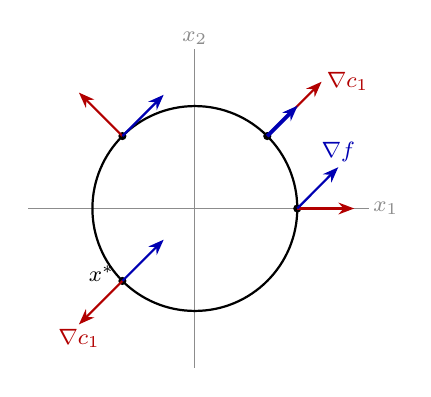
\begin{tikzpicture}[scale=0.92]
        \draw[black!45] (-2.3,0)--(2.4,0) node[lab,right]{$x_{1}$};
        \draw[black!45] (0,-2.2)--(0,2.2) node[lab,above]{$x_{2}$};
        \draw[thick] (0,0) circle (1.414);
        \foreach \px/\py in {-1/-1,1/1,-1/1,1.414/0}{\fill (\px,\py) circle (1.6pt);}
        % gradients of f (blue) and c1 (red)
        \draw[vec,blue!70!black] (-1,-1)--(-0.43,-0.43);
        \draw[vec,red!70!black] (-1,-1)--(-1.6,-1.6) node[lab,below]{$\nabla c_{1}$};
        \node[lab,left] at (-1.05,-0.9) {$\xs$};
        \draw[vec,red!70!black] (1,1)--(1.75,1.75) node[lab,right]{$\nabla c_{1}$};
        \draw[vec,blue!70!black,line width=1.4pt] (1,1)--(1.42,1.42);
        \draw[vec,red!70!black] (-1,1)--(-1.6,1.6);
        \draw[vec,blue!70!black] (-1,1)--(-0.43,1.57);
        \draw[vec,red!70!black] (1.414,0)--(2.2,0);
        \draw[vec,blue!70!black] (1.414,0)--(1.98,0.57) node[lab,above]{$\gradf$};
      \end{tikzpicture}
    \end{column}
  \end{columns}
\end{frame}

\begin{frame}{Example 12.1: where (12.10) comes from}
  Conjecture: a feasible $x$ is not optimal if there is a small step $s$ that retains feasibility and
  decreases $f$. Use first-order Taylor series for $c_{1}$ and $f$.
  \begin{itemize}\setlength\itemsep{0.6em}
    \item \textbf{Feasibility.} We need $c_{1}(x+s)=0$. Since $x$ is feasible, $c_{1}(x)=0$, so
      \[ 0=c_{1}(x+s)\approx c_{1}(x)+\nabla c_{1}(x)^{T}s=\nabla c_{1}(x)^{T}s . \tag{12.11} \]
      To first order, $s$ retains feasibility when
      \[ \nabla c_{1}(x)^{T}s=0 . \tag{12.12} \]
    \item \textbf{Decrease.} We need $0>f(x+s)-f(x)\approx\gradf(x)^{T}s$. To first order,
      \[ \gradf(x)^{T}s<0 . \tag{12.13} \]
  \end{itemize}
  \readbook{p.~309 (through (12.15)).}
\end{frame}

\begin{frame}{Example 12.1: the direction $d$ in (12.14)}
  If a small $s$ satisfies (12.12) and (12.13), then $d\approx s/\|s\|$ (not small) satisfies
  \[ \nabla c_{1}(x)^{T}d=0\quad\text{and}\quad\gradf(x)^{T}d<0 . \tag{12.14} \]
  If no direction $d$ satisfies (12.14), it is likely that no such step $s$ exists.
  Then $x$ appears to be a local minimizer.
  \begin{columns}[T,totalwidth=\textwidth]
    \begin{column}{0.64\textwidth}
      \vspace{0.3em}
      (12.14): $d$ is orthogonal to $\nabla c_{1}(x)$ and has a negative inner product with $\gradf(x)$.

      \vspace{0.6em}
      \textbf{Parallel case}, $\gradf(x)=\lambda_{1}\nabla c_{1}(x)$:\\ every $d$ with
      $\nabla c_{1}(x)^{T}d=0$ has
      \[ \gradf(x)^{T}d=\lambda_{1}\nabla c_{1}(x)^{T}d=0 . \]
      No $d$ satisfies (12.14).
    \end{column}
    \begin{column}{0.34\textwidth}
      \centering
      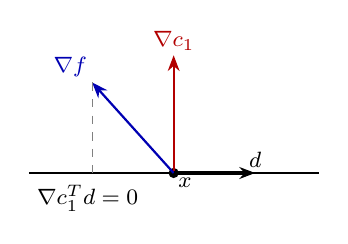
\begin{tikzpicture}[scale=1.15]
        \draw[thick] (-1.6,0)--(1.6,0);
        \node[lab] at (-0.95,-0.28) {$\nabla c_{1}^{T}d=0$};
        \fill (0,0) circle (1.6pt) node[lab,below right]{$x$};
        \draw[vec,red!70!black] (0,0)--(0,1.3) node[lab,above]{$\nabla c_{1}$};
        \draw[vec,blue!70!black] (0,0)--(-0.9,1.0) node[lab,above left]{$\gradf$};
        \draw[dashed,black!50] (-0.9,1.0)--(-0.9,0);
        \draw[vec,line width=1.3pt] (0,0)--(0.9,0) node[lab,above]{$d$};
      \end{tikzpicture}

      {\small Not parallel: a $d$ satisfying (12.14) exists.}
    \end{column}
  \end{columns}
\end{frame}

\begin{frame}{Example 12.1: $\gradf(x)$ and $\nabla c_{1}(x)$ not parallel}
  Remove from $-\gradf(x)$ its component along $\nabla c_{1}(x)$:
  \[ \bar d=-\Bigl(I-\frac{\nabla c_{1}(x)\nabla c_{1}(x)^{T}}{\|\nabla c_{1}(x)\|^{2}}\Bigr)\gradf(x),
     \qquad d=\frac{\bar d}{\|\bar d\|} . \tag{12.15} \]
  \begin{itemize}\setlength\itemsep{0.35em}
    \item $\bar d\ne 0$, because $\gradf(x)$ is not a multiple of $\nabla c_{1}(x)$.
    \item $\nabla c_{1}(x)^{T}\bar d=0$ and $\gradf(x)^{T}\bar d=-\|\bar d\|^{2}<0$:
      $d$ satisfies (12.14) (Exercise 12.7).
    \item Conclusion: no $d$ satisfies (12.14) only if $\gradf(x)=\lambda_{1}\nabla c_{1}(x)$
      for some scalar $\lambda_{1}$.
    \item At $x=(\sqrt2,0)^{T}$: $\gradf=(1,1)^{T}$, $\nabla c_{1}=(2\sqrt2,0)^{T}$, and (12.15) gives
      $d=(0,-1)^{T}$, the clockwise direction.
    \item At $\xs=(-1,-1)^{T}$: $\gradf=(1,1)^{T}$, $\nabla c_{1}=(-2,-2)^{T}$, so
      $\gradf(\xs)=-\tfrac12\nabla c_{1}(\xs)$. This is (12.10).
  \end{itemize}
\end{frame}

\begin{frame}{Example 12.1: the Lagrangian function}
  \textbf{Lagrangian function}:
  \[ \cL(x,\lambda_{1})=f(x)-\lambda_{1}c_{1}(x) . \tag{12.16} \]
  Since $\nabla_{x}\cL(x,\lambda_{1})=\gradf(x)-\lambda_{1}\nabla c_{1}(x)$, condition (12.10) is:
  at the solution $\xs$ there is a scalar $\ls_{1}$ such that
  $\nabla_{x}\cL(\xs,\ls_{1})=0$ \eqn{12.17}.
  \begin{itemize}\setlength\itemsep{0.4em}
    \item We can search for solutions of (12.9) among the stationary points of $\cL$.
      $\lambda_{1}$ is the \textbf{Lagrange multiplier} for the constraint $c_{1}(x)=0$.
    \item Necessary, not sufficient: (12.10) holds at $x=(1,1)^{T}$ with $\lambda_{1}=\tfrac12$.
      This point maximizes $f$ on the circle.
    \item No sign condition on $\lambda_{1}$ makes (12.10) sufficient. Replace the constraint by
      $2-x_{1}^{2}-x_{2}^{2}=0$: the solution is not affected, and $\ls_{1}$ changes from
      $-\tfrac12$ to $\tfrac12$.
  \end{itemize}
  \readbook{p.~310.}
\end{frame}

\begin{frame}{Example 12.2 (a single inequality constraint)}
  \begin{columns}[T,totalwidth=\textwidth]
    \begin{column}{0.66\textwidth}
      \[ \min\ x_{1}+x_{2}\quad\text{s.t.}\quad 2-x_{1}^{2}-x_{2}^{2}\ge 0 \tag{12.18} \]
      Solution $(-1,-1)^{T}$; (12.10) holds with $\ls_{1}=\tfrac12$.\\
      Feasibility to first order: $c_{1}(x)+\nabla c_{1}(x)^{T}s\ge 0$ \eqn{12.19}.

      \vspace{0.15em}
      \textbf{Case I}, $c_{1}(x)>0$: every small $s$ satisfies (12.19). A feasible
      descent step exists unless $\gradf(x)=0$ \eqn{12.20}.

      \vspace{0.15em}
      \textbf{Case II}, $c_{1}(x)=0$: need $\gradf(x)^{T}s<0$ and $\nabla c_{1}(x)^{T}s\ge 0$.
      The intersection of the two half-spaces is empty only when
      $\gradf(x)=\lambda_{1}\nabla c_{1}(x)$ for some $\lambda_{1}\ge 0$ \eqn{12.21}.
      With $\lambda_{1}<0$ the two conditions hold on an open half-plane.
    \end{column}
    \begin{column}{0.32\textwidth}
      \centering
      \begin{tikzpicture}[scale=1.08]
        \fill[black!6] (0,0) circle (1.5);
        \draw[thick] (0,0) circle (1.5);
        % interior point (Case I)
        \fill (0.5,-0.45) circle (1.6pt);
        \draw[vec,blue!70!black] (0.5,-0.45)--(0.95,0.0) node[lab,above]{$\gradf$};
        \draw[vec] (0.5,-0.45)--(0.1,-0.85) node[lab,left]{$s$};
        % boundary point (Case II), angle 160 degrees
        \fill[structure!45] (-1.41,0.51)--++(-110:0.95) arc (-110:-45:0.95)--cycle;
        \fill (-1.41,0.51) circle (1.6pt);
        \draw[vec,red!70!black] (-1.41,0.51)--++(-20:0.85) node[lab,right]{$\nabla c_{1}$};
        \draw[vec,blue!70!black] (-1.41,0.51)--++(45:0.75) node[lab,right]{$\gradf$};
        \node[lab] at (0,-1.85) {Interior point: Case I.};
        \node[lab] at (0,-2.25) {Boundary point: Case II;};
        \node[lab] at (0,-2.65) {the shaded $s$ satisfy both.};
      \end{tikzpicture}
    \end{column}
  \end{columns}
\end{frame}

\begin{frame}{Complementarity; Example 12.3 (two inequality constraints)}
  Cases I and II together: when no first-order feasible descent direction exists at $\xs$,
  \[ \nabla_{x}\cL(\xs,\ls_{1})=0\ \ \text{for some }\ls_{1}\ge 0\ \ \eqn{12.22},\qquad\quad
     \ls_{1}\,c_{1}(\xs)=0\ \ \eqn{12.23}. \]
  (12.23) is a \textbf{complementarity condition}: $\lambda_{1}$ can be strictly positive only when
  $c_{1}$ is active.

  \vspace{0.4em}
  \textbf{Example 12.3.}\ \ $\min\ x_{1}+x_{2}$\ \ s.t.\ \ $2-x_{1}^{2}-x_{2}^{2}\ge 0,\ \ x_{2}\ge 0$ \eqn{12.24}.

  \begin{center}\small\setlength\tabcolsep{5pt}
  \begin{tabular}{llll}
    \toprule
    Point $x$ & $\cA(x)$ & $\lambda$ from $\nabla_{x}\cL=0$, (12.27) & Conclusion \\
    \midrule
    $(-\sqrt2,0)^{T}$ & $\{1,2\}$ & $\bigl(\tfrac{1}{2\sqrt2},\,1\bigr)^{T}$ & $\lambda\ge 0$: the solution \\[0.2em]
    $(\sqrt2,0)^{T}$ & $\{1,2\}$ & $\bigl(-\tfrac{1}{2\sqrt2},\,1\bigr)^{T}$ & $\lambda_{1}<0$; $d=(-1,0)^{T}$ satisfies (12.25) \\[0.2em]
    $(1,0)^{T}$ & $\{2\}$ & $\lambda_{1}=0$, no $\lambda_{2}$ exists & $d=(-\tfrac12,\tfrac14)^{T}$ satisfies (12.28) \\
    \bottomrule
  \end{tabular}
  \end{center}
  \readbook{pp.~313--315.}
\end{frame}

%=====================================================================
\section{\S12.2 Tangent cone and constraint qualifications}

\begin{frame}{Tangent cone and linearized feasible directions}
  \textbf{Feasible sequence approaching $x$}: $z_{k}\in\Omega$ for all $k$ sufficiently large and $z_{k}\to x$.
  \begin{block}{Definition 12.2}
    The vector $d$ is a \textbf{tangent} to $\Omega$ at $x$ if there are a feasible sequence $\{z_{k}\}$
    approaching $x$ and a sequence of positive scalars $\{t_{k}\}$ with $t_{k}\to 0$ such that
    $\lim_{k\to\infty}(z_{k}-x)/t_{k}=d$ \eqn{12.29}.
    The set of all tangents to $\Omega$ at $\xs$ is the \textbf{tangent cone} $\TO(\xs)$.
  \end{block}
  \begin{block}{Definition 12.3}
    The set of \textbf{linearized feasible directions} at a feasible $x$ is
    \[ \cF(x)=\bigl\{d\ \bigm|\ d^{T}\nabla c_{i}(x)=0\ \ \forall i\in\cE,\quad
       d^{T}\nabla c_{i}(x)\ge 0\ \ \forall i\in\cA(x)\cap\cI\bigr\} . \]
  \end{block}
  $\TO(x)$: geometry of $\Omega$ only.\ \ $\cF(x)$: depends on the functions $c_{i}$.\ \ \readbook{p.~316.}
\end{frame}

\begin{frame}{$\TO(x)$ and $\cF(x)$ in the examples}
  \begin{center}\small\setlength\tabcolsep{5pt}
  \begin{tabular}{llll}
    \toprule
    Constraints & $x$ & $\TO(x)$ & $\cF(x)$ \\
    \midrule
    (12.9):\ \ $x_{1}^{2}+x_{2}^{2}-2=0$ & $(-\sqrt2,0)^{T}$ & $\{(0,d_{2})^{T}\}$ & $\{(0,d_{2})^{T}\}$ \\[0.15em]
    (12.31):\ \ $(x_{1}^{2}+x_{2}^{2}-2)^{2}=0$ & $(-\sqrt2,0)^{T}$ & $\{(0,d_{2})^{T}\}$ & $\R^{2}$ \\[0.15em]
    (12.18):\ \ $2-x_{1}^{2}-x_{2}^{2}\ge 0$ & $(-\sqrt2,0)^{T}$ & $\{w\mid w_{1}\ge 0\}$ & $\{d\mid d_{1}\ge 0\}$ \\[0.15em]
    (12.32):\ \ $1-x_{1}^{2}-(x_{2}-1)^{2}\ge 0,\ \ -x_{2}\ge 0$ & $(0,0)^{T}$ & $\{(0,0)^{T}\}$ & $\{(d_{1},0)^{T}\}$ \\
    \bottomrule
  \end{tabular}
  \end{center}
  \begin{columns}[T,totalwidth=\textwidth]
    \begin{column}{0.68\textwidth}
      \begin{itemize}\setlength\itemsep{0.3em}
        \item (12.9) and (12.31) define the same set $\Omega$. In (12.31), $\nabla c_{1}(x)=0$ on $\Omega$,
          so every $d$ is in $\cF(x)$.
        \item (12.32): $\Omega$ is the single point $(0,0)^{T}$, but $\cF(x)$ is the entire horizontal axis.
        \item Conditions on $\gradf$ and $\nabla c_{i}$ describe $\Omega$ near $x$ only if $\cF(x)$
          is similar to $\TO(x)$.
      \end{itemize}
      \vspace{0.2em}
    \end{column}
    \begin{column}{0.30\textwidth}
      \centering
      \begin{tikzpicture}[scale=0.85]
        \fill[black!10] (-1.7,-0.7) rectangle (1.7,0);
        \fill[structure!30] (0,1) circle (1);
        \draw[thick] (0,1) circle (1);
        \draw[thick] (-1.7,0)--(1.7,0);
        \fill (0,0) circle (1.8pt);
        \node[lab] at (0,1) {$c_{1}\ge 0$};
        \node[lab] at (-0.9,-0.38) {$c_{2}\ge 0$};
        \node[lab,below] at (0.35,0) {$x$};
        \node[lab] at (0,-1.05) {(12.32)};
      \end{tikzpicture}
    \end{column}
  \end{columns}
  \readbook{Examples 12.4 and 12.5, pp.~317--320.}
\end{frame}

\begin{frame}{Constraint qualifications; LICQ}
  \textbf{Constraint qualifications}: conditions under which $\cF(x)$ is similar to $\TO(x)$.
  Most of them ensure that the two sets are identical.
  \begin{block}{Definition 12.4 (LICQ)}
    Given the point $x$ and the active set $\cA(x)$, the \textbf{linear independence constraint
    qualification} holds if the set of active constraint gradients
    $\{\nabla c_{i}(x),\ i\in\cA(x)\}$ is linearly independent.
  \end{block}
  \begin{itemize}\setlength\itemsep{0.25em}
    \item LICQ fails in (12.31): $\nabla c_{1}(x)=0$. It fails in (12.32):
      $\nabla c_{1}(x)=(0,2)^{T}$, $\nabla c_{2}(x)=(0,-1)^{T}$.
    \item Lemma 12.7: if all active constraints at $\xs$ are linear, then $\cF(\xs)=\TO(\xs)$.
    \item MFCQ (Definition 12.6) is weaker than LICQ. Theorem 12.1 also holds with MFCQ;
      the set of multipliers $\ls$ is then bounded, not necessarily a single vector.
  \end{itemize}
  \readbook{\S12.6, pp.~338--340.}
\end{frame}

%=====================================================================
\section{\S12.3 First-order optimality conditions}

\begin{frame}{Theorem 12.1: the KKT conditions}
  Lagrangian for (12.1):\quad
  $\cL(x,\lambda)=f(x)-\sum_{i\in\cE\cup\cI}\lambda_{i}c_{i}(x)$ \eqn{12.33}.
  \begin{block}{Theorem 12.1 (First-Order Necessary Conditions)}
    \small Suppose that $\xs$ is a local solution of (12.1), that the functions $f$ and $c_{i}$ in (12.1) are
    continuously differentiable, and that the LICQ holds at $\xs$. Then there is a Lagrange multiplier
    vector $\ls$, with components $\ls_{i}$, $i\in\cE\cup\cI$, such that the following conditions are
    satisfied at $(\xs,\ls)$:
    \vspace{-0.8em}
    \begin{align}
      \nabla_{x}\cL(\xs,\ls) &= 0, \tag{12.34a}\\[-0.35em]
      c_{i}(\xs) &= 0\quad\text{for all } i\in\cE, \tag{12.34b}\\[-0.35em]
      c_{i}(\xs) &\ge 0\quad\text{for all } i\in\cI, \tag{12.34c}\\[-0.35em]
      \ls_{i} &\ge 0\quad\text{for all } i\in\cI, \tag{12.34d}\\[-0.35em]
      \ls_{i}\,c_{i}(\xs) &= 0\quad\text{for all } i\in\cE\cup\cI. \tag{12.34e}
    \end{align}
  \end{block}
  (12.34): the \textbf{Karush--Kuhn--Tucker (KKT) conditions}.
\end{frame}

\begin{frame}{Remarks on the KKT conditions; Example 12.6}
  \begin{itemize}\setlength\itemsep{0.25em}
    \item (12.34e), complementarity: constraint $i$ is active, or $\ls_{i}=0$, or both. Multipliers of
      inactive inequalities are zero, so (12.34a) is
      \[ 0=\nabla_{x}\cL(\xs,\ls)=\gradf(\xs)-\sum_{i\in\cA(\xs)}\ls_{i}\nabla c_{i}(\xs) . \tag{12.35} \]
    \item Definition 12.5 (\textbf{strict complementarity}): exactly one of $\ls_{i}$ and $c_{i}(\xs)$
      is zero for each $i\in\cI$; that is, $\ls_{i}>0$ for each $i\in\cI\cap\cA(\xs)$.
    \item When the LICQ holds, the optimal $\ls$ is unique (Exercise 12.17).
    \item Example 12.6: $\min\,(x_{1}-\tfrac32)^{2}+(x_{2}-\tfrac12)^{4}$ subject to the constraints
      (12.6) \eqn{12.36}. At $\xs=(1,0)^{T}$,
      $c_{1}=1-x_{1}-x_{2}$ and $c_{2}=1-x_{1}+x_{2}$ are active:
      $\gradf=(-1,-\tfrac12)^{T}$, $\nabla c_{1}=(-1,-1)^{T}$, $\nabla c_{2}=(-1,1)^{T}$,
      $\ls=(\tfrac34,\tfrac14,0,0)^{T}$.
  \end{itemize}
  \readbook{pp.~321--322.}
\end{frame}

%=====================================================================
\section{\S12.4 First-order optimality conditions: proof}

\begin{frame}{Proof of Theorem 12.1, first result: Lemma 12.2}
  Rows of $A(\xs)$: the active constraint gradients,
  $A(\xs)^{T}=[\nabla c_{i}(\xs)]_{i\in\cA(\xs)}$ \eqn{12.37}.
  \begin{block}{Lemma 12.2}
    Let $\xs$ be a feasible point. The following two statements are true.
    \begin{itemize}
      \item[(i)] $\TO(\xs)\subset\cF(\xs)$.
      \item[(ii)] If the LICQ condition is satisfied at $\xs$, then $\cF(\xs)=\TO(\xs)$.
    \end{itemize}
  \end{block}
  \begin{itemize}\setlength\itemsep{0.25em}
    \item (i): Taylor's theorem for $c_{i}(z_{k})$, $z_{k}=\xs+t_{k}d+o(t_{k})$ \eqn{12.38}.
      No constraint qualification.\vspace{-0.15em}
    \item (ii): for $d\in\cF(\xs)$, the implicit function theorem applied to (12.40) gives a feasible
      sequence with limiting direction $d$. The Jacobian (12.41) is nonsingular because $A(\xs)$
      has full row rank. \alert{The LICQ is used here.}
  \end{itemize}
  \readbook{proof of Lemma 12.2(i), pp.~323--324.} Proof of (ii): pp.~324--325.
\end{frame}

\begin{frame}{Second result: Theorem 12.3}
  \begin{block}{Theorem 12.3}
    If $\xs$ is a local solution of (12.1), then we have
    \[ \gradf(\xs)^{T}d\ge 0\quad\text{for all } d\in\TO(\xs) . \tag{12.43} \]
  \end{block}
  \begin{itemize}\setlength\itemsep{0.35em}
    \item No constraint qualification. The statement uses $\TO(\xs)$, not $\cF(\xs)$.
    \item Idea of the proof: if $\gradf(\xs)^{T}d<0$ for a tangent $d$, then along its feasible sequence
      $f(z_{k})<f(\xs)+\tfrac12 t_{k}\,d^{T}\gradf(\xs)$ for all $k$ sufficiently large.
    \item The converse is not true:\ \ $\min\ x_{2}$\ \ subject to\ \ $x_{2}\ge -x_{1}^{2}$ \eqn{12.44}.
      At $\xs=(0,0)^{T}$ every tangent has $d_{2}\ge 0$, so $\gradf(\xs)^{T}d=d_{2}\ge 0$. But
      $(\alpha,-\alpha^{2})^{T}$ is feasible with a smaller $f$ for every $\alpha>0$.
  \end{itemize}
  \readbook{proof of Theorem 12.3, pp.~325--326.}
\end{frame}

\begin{frame}{Third result: Farkas' Lemma}
  \begin{columns}[T,totalwidth=\textwidth]
    \begin{column}{0.56\textwidth}
      Cone: $K=\{By+Cw\mid y\ge 0\}$ \eqn{12.45},\\
      with $B\in\R^{n\times m}$ and $C\in\R^{n\times p}$.
      \begin{block}{Lemma 12.4 (Farkas)}
        Let the cone $K$ be defined as in (12.45). Given any vector $g\in\R^{n}$, we have either that
        $g\in K$ or that there exists $d\in\R^{n}$ satisfying
        \[ g^{T}d<0,\quad B^{T}d\ge 0,\quad C^{T}d=0, \tag{12.46} \]
        but not both.
      \end{block}
    \end{column}
    \begin{column}{0.42\textwidth}
      \centering
      \begin{tikzpicture}[scale=0.78]
        % left panel: g in K
        \fill[structure!25] (0,0)--(30:1.9)--(150:1.9)--cycle;
        \draw[vec] (0,0)--(150:1.6) node[lab,above]{$b_{1}$};
        \draw[vec] (0,0)--(110:1.1) node[lab,above]{$b_{2}$};
        \draw[vec] (0,0)--(30:1.6) node[lab,above]{$b_{3}$};
        \draw[vec,blue!70!black] (0,0)--(68:1.35) node[lab,above]{$g$};
        \node[lab] at (0,-0.45) {$g\in K$};
        % right panel: separating hyperplane
        \begin{scope}[xshift=3.7cm]
          \fill[structure!25] (0,0)--(30:1.9)--(150:1.9)--cycle;
          \draw[vec] (0,0)--(150:1.6) node[lab,above]{$b_{1}$};
          \draw[vec] (0,0)--(95:1.1) node[lab,above]{$b_{2}$};
          \draw[vec] (0,0)--(30:1.6) node[lab,above]{$b_{3}$};
          \draw[dashed] (-1.7,0)--(1.7,0);
          \draw[vec,blue!70!black] (0,0)--(-25:1.35) node[lab,right]{$g$};
          \draw[vec,red!70!black] (0,0)--(90:0.6);
          \node[lab,red!70!black] at (0.22,0.42) {$d$};
          \node[lab] at (0,-1.05) {$g\notin K$};
        \end{scope}
      \end{tikzpicture}

      \vspace{0.2em}
      {\small $n=2$, $B=[b_{1}\ b_{2}\ b_{3}]$, $C$ null.\\
      Dashed: the hyperplane $d^{T}x=0$.}
    \end{column}
  \end{columns}
  Proof for $g\notin K$: $d=\hat s-g$, where $\hat s$ is the vector in $K$ closest to $g$ \eqn{12.47}.
  It needs $K$ to be closed.\\[0.3em]
  \readbook{proof of Lemma 12.4, pp.~327--328; Lemma 12.15 ($K$ is closed), pp.~350--351.}
\end{frame}

\begin{frame}{Proof of Theorem 12.1: putting the three results together}
  Apply Lemma 12.4 with $g=\gradf(\xs)$ and the cone
  \[ N=\Bigl\{\sum_{i\in\cA(\xs)}\lambda_{i}\nabla c_{i}(\xs),\quad
      \lambda_{i}\ge 0\ \text{for } i\in\cA(\xs)\cap\cI\Bigr\} . \tag{12.50} \]
  The second alternative (12.46) is then: $d^{T}\gradf(\xs)<0$ and $d\in\cF(\xs)$.
  \begin{enumerate}\setlength\itemsep{0.1em}
    \item Theorem 12.3: $d^{T}\gradf(\xs)\ge 0$ for all $d\in\TO(\xs)$.
    \item Lemma 12.2(ii), \alert{LICQ}: $\TO(\xs)=\cF(\xs)$. So $d^{T}\gradf(\xs)\ge 0$ for all $d\in\cF(\xs)$.
    \item Lemma 12.4: the second alternative cannot hold, so $\gradf(\xs)\in N$. This is (12.51):
      $\gradf(\xs)=\sum_{i\in\cA(\xs)}\lambda_{i}\nabla c_{i}(\xs)$ with
      $\lambda_{i}\ge 0$ for $i\in\cA(\xs)\cap\cI$.
    \item Define $\ls_{i}=\lambda_{i}$ for $i\in\cA(\xs)$ and $\ls_{i}=0$ for $i\in\cI\backslash\cA(\xs)$
      \eqn{12.52}. Then (12.34a)--(12.34e) hold.
  \end{enumerate}
  \readbook{proof of Theorem 12.1, p.~329.}
\end{frame}

%=====================================================================
\section{\S12.5 Second-order conditions}

\begin{frame}{The critical cone}
  \S12.5: $f$, $c_{i}$ twice continuously differentiable. For $w\in\cF(\xs)$ with
  $w^{T}\gradf(\xs)=0$, first derivatives do not determine whether $f$ increases or decreases along $w$.
  \[ w\in\cC(\xs,\ls)\ \Leftrightarrow\
     \begin{cases}
       \nabla c_{i}(\xs)^{T}w=0, & \text{for all } i\in\cE,\\
       \nabla c_{i}(\xs)^{T}w=0, & \text{for all } i\in\cA(\xs)\cap\cI \text{ with } \ls_{i}>0,\\
       \nabla c_{i}(\xs)^{T}w\ge 0, & \text{for all } i\in\cA(\xs)\cap\cI \text{ with } \ls_{i}=0.
     \end{cases} \tag{12.53} \]
  \textbf{Critical cone} $\cC(\xs,\ls)$. From (12.34a):\ \
  $w\in\cC(\xs,\ls)\ \Rightarrow\ w^{T}\gradf(\xs)=0$ \eqn{12.55}.

  \vspace{0.3em}
  \textbf{Example 12.7.}\ \ $\min\ x_{1}$\ \ s.t.\ \ $x_{2}\ge 0,\ \ 1-(x_{1}-1)^{2}-x_{2}^{2}\ge 0$ \eqn{12.56}.
  \begin{columns}[T,totalwidth=\textwidth]
    \begin{column}{0.72\textwidth}
      $\xs=(0,0)^{T}$, $\cA(\xs)=\{1,2\}$, $\ls=(0,0.5)^{T}$.\\
      $\cF(\xs)=\{d\mid d\ge 0\}$,\ \ $\cC(\xs,\ls)=\{(0,w_{2})^{T}\mid w_{2}\ge 0\}$.
      \readbook{pp.~330--331.}
    \end{column}
    \begin{column}{0.26\textwidth}
      \centering
      \begin{tikzpicture}[scale=0.85]
        \fill[black!8] (0,0) rectangle (2.1,1.25);
        \begin{scope}
          \clip (-0.2,0) rectangle (2.2,1.3);
          \fill[structure!35] (1,0) circle (1);
          \draw[thick] (1,0) circle (1);
        \end{scope}
        \draw[thick] (0,0)--(2.1,0);
        \draw[line width=1.6pt,red!70!black] (0,0)--(0,1.25) node[lab,left]{$\cC$};
        \draw[vec,blue!70!black] (0,0)--(-0.8,0) node[lab,below]{$-\gradf$};
        \fill (0,0) circle (1.8pt);
        \node[lab] at (1.65,1.02) {$\cF$};
        \node[lab] at (1,0.4) {$\Omega$};
      \end{tikzpicture}
    \end{column}
  \end{columns}
\end{frame}

\begin{frame}{Theorem 12.5: second-order necessary conditions}
  \begin{block}{Theorem 12.5 (Second-Order Necessary Conditions)}
    Suppose that $\xs$ is a local solution of (12.1) and that the LICQ condition is satisfied. Let $\ls$
    be the Lagrange multiplier vector for which the KKT conditions (12.34) are satisfied. Then
    \[ w^{T}\hessL(\xs,\ls)\,w\ge 0\quad\text{for all } w\in\cC(\xs,\ls) . \tag{12.57} \]
  \end{block}
  \begin{itemize}\setlength\itemsep{0.3em}
    \item The matrix is $\hessL=\hessf-\sum_{i}\ls_{i}\nabla^{2}c_{i}$, not $\hessf$.
      The inequality is required only for $w$ in the critical cone.
    \item Proof: a feasible sequence with limiting direction $w\in\cC(\xs,\ls)$, built as in
      Lemma 12.2(ii), has $f(z_{k})=f(\xs)+\tfrac12 t_{k}^{2}\,w^{T}\hessL(\xs,\ls)\,w+o(t_{k}^{2})$ \eqn{12.64}.
      See pp.~332--333.
  \end{itemize}
\end{frame}

\begin{frame}{Theorem 12.6: second-order sufficient conditions}
  \begin{block}{Theorem 12.6 (Second-Order Sufficient Conditions)}
    Suppose that for some feasible point $\xs\in\R^{n}$ there is a Lagrange multiplier vector $\ls$
    such that the KKT conditions (12.34) are satisfied. Suppose also that
    \[ w^{T}\hessL(\xs,\ls)\,w>0\quad\text{for all } w\in\cC(\xs,\ls),\ w\ne 0 . \tag{12.65} \]
    Then $\xs$ is a strict local solution for (12.1).
  \end{block}
  \begin{itemize}\setlength\itemsep{0.35em}
    \item No constraint qualification is required. The inequality in (12.57) is now strict.
    \item The proof shows more: every feasible sequence $\{z_{k}\}$ approaching $\xs$ has
      $f(z_{k})\ge f(\xs)+(\sigma/4)\|z_{k}-\xs\|^{2}$ for all $k$ sufficiently large. Here $\sigma>0$ is
      the minimum of $d^{T}\hessL(\xs,\ls)\,d$ over $\{d\in\cC(\xs,\ls)\mid\|d\|=1\}$.
  \end{itemize}
  \readbook{proof of Theorem 12.6, pp.~333--335.}
\end{frame}

\begin{frame}{Examples 12.8 and 12.9}
  \textbf{Example 12.8.} Problem (12.18): $\xs=(-1,-1)^{T}$, $\ls_{1}=\tfrac12$,
  $\hessL(\xs,\ls)=2\ls_{1}I=I$ is positive definite: strict local solution.

  \vspace{0.4em}
  \textbf{Example 12.9.}\ \ $\min\ -0.1(x_{1}-4)^{2}+x_{2}^{2}$\ \ s.t.\ \ $x_{1}^{2}+x_{2}^{2}-1\ge 0$ \eqn{12.72}.
  \begin{itemize}\setlength\itemsep{0.2em}
    \item $f$ is not bounded below on the feasible region: no global solution.
    \item $\hessL(x,\lambda)=\mathrm{diag}(-0.2-2\lambda_{1},\ 2-2\lambda_{1})$ \eqn{12.73b}.
    \item $\xs=(1,0)^{T}$ satisfies the KKT conditions with $\ls_{1}=0.3$ and $\cA(\xs)=\{1\}$.
    \item $\nabla c_{1}(\xs)=(2,0)^{T}$: $\cC(\xs,\ls)=\{(0,w_{2})^{T}\mid w_{2}\in\R\}$,
      $w^{T}\hessL(\xs,\ls)\,w=1.4\,w_{2}^{2}>0$.
    \item $\hessL(\xs,\ls)=\mathrm{diag}(-0.8,\,1.4)$ is indefinite. Its negative-curvature direction
      $(1,0)^{T}$ is not in $\cC(\xs,\ls)$. So $(1,0)^{T}$ is a strict local solution.
  \end{itemize}
  {\small (The book prints $-0.4$ on p.~336; (12.73b) gives $-0.8$. Same conclusion.)}
\end{frame}

\begin{frame}{Second-order conditions and projected Hessians}
  Suppose $\ls$ is unique (for example, the LICQ holds) and strict complementarity holds.
  Then (12.53) reduces to
  \[ \cC(\xs,\ls)=\mathrm{Null}\,\bigl[\nabla c_{i}(\xs)^{T}\bigr]_{i\in\cA(\xs)}=\mathrm{Null}\,A(\xs) . \]
  Let $Z$ have full column rank with columns that span $\cC(\xs,\ls)$. Then
  \begin{itemize}\setlength\itemsep{0.3em}
    \item (12.57) in Theorem 12.5\ \ $\Leftrightarrow$\ \ $Z^{T}\hessL(\xs,\ls)Z$ is positive semidefinite;
    \item (12.65) in Theorem 12.6\ \ $\Leftrightarrow$\ \ $Z^{T}\hessL(\xs,\ls)Z$ is positive definite.
  \end{itemize}
  $Z$ can be computed from a QR factorization of $A(\xs)^{T}$:
  \[ A(\xs)^{T}=Q\begin{bmatrix}R\\0\end{bmatrix}
     =\begin{bmatrix}Q_{1} & Q_{2}\end{bmatrix}\begin{bmatrix}R\\0\end{bmatrix}=Q_{1}R . \tag{12.74} \]
  If $R$ is nonsingular, set $Z=Q_{2}$.\ \ In Example 12.9: $A(\xs)=[\,2\ \ 0\,]$, $Z=(0,1)^{T}$,
  $Z^{T}\hessL Z=1.4$.

  \vspace{0.3em}
  \readbook{p.~337.}
\end{frame}

%=====================================================================
\section{\S12.7 A geometric viewpoint}

\begin{frame}{The normal cone}
  \textbf{Normal cone} to $\Omega$ at $x\in\Omega$ (Definition 12.7):
  \[ \NO(x)=\{v\mid v^{T}w\le 0\ \text{for all } w\in\TO(x)\} . \tag{12.77} \]
  \begin{block}{Theorem 12.8}
    Suppose that $\xs$ is a local minimizer of $f$ in $\Omega$. Then\ \
    $-\gradf(\xs)\in\NO(\xs)$ \eqn{12.78}.
  \end{block}
  \begin{itemize}\setlength\itemsep{0.3em}
    \item (12.78) depends only on the geometry of $\Omega$, not on the functions $c_{i}$.
      It is Theorem 12.3 written with Definition 12.7.
    \item Lemma 12.9: if the LICQ holds at $\xs$, then $\NO(\xs)=-N$ with $N$ from (12.50).
      Then (12.78) is (12.51).
  \end{itemize}
  \readbook{pp.~340--341.}
\end{frame}

%=====================================================================
\section{\S12.8 Lagrange multipliers and sensitivity}

\begin{frame}{Lagrange multipliers and sensitivity}
  Perturb an active constraint $i$: require $c_{i}(x)\ge-\epsilon\|\nabla c_{i}(\xs)\|$ instead of
  $c_{i}(x)\ge 0$. Suppose $\epsilon$ is small enough that the perturbed solution $\xs(\epsilon)$ has
  the same active set and the multipliers are not much affected. Then
  \[ \frac{d f(\xs(\epsilon))}{d\epsilon}=-\ls_{i}\,\|\nabla c_{i}(\xs)\| . \tag{12.80} \]
  \begin{itemize}\setlength\itemsep{0.25em}
    \item The derivation is informal. It can be made rigorous with strict complementarity and
      second-order conditions.
    \item Definition 12.8: $c_{i}$ is \textbf{strongly active} (\textbf{binding}) if $i\in\cA(\xs)$ and
      $\ls_{i}>0$ for some $\ls$ satisfying (12.34); \textbf{weakly active} if $i\in\cA(\xs)$ and
      $\ls_{i}=0$ for all such $\ls$.
    \item Replacing $c_{i}$ by $10c_{i}$ gives $\ls_{i}/10$ and $10\nabla c_{i}(\xs)$:
      (12.80) does not change.
  \end{itemize}
  \readbook{pp.~341--343.}
\end{frame}

\begin{frame}{Example: dispatch of two generators {\normalfont\small(Not in the book.)}}
  Outputs $p_{1},p_{2}$, demand $3$, limit $p_{1}\le 1.5$:
  \[ \min\ p_{1}^{2}+2p_{2}^{2}\quad\text{s.t.}\quad c_{1}(p)=p_{1}+p_{2}-3=0,\qquad c_{2}(p)=1.5-p_{1}\ge 0 . \]
  (12.34a):\ \ $2p_{1}-\lambda_{1}+\lambda_{2}=0$,\ \ $4p_{2}-\lambda_{1}=0$.
  \begin{itemize}\setlength\itemsep{0.25em}
    \item Without $c_{2}$: $p=(2,1)^{T}$, $\lambda_{1}=4$.
    \item With $c_{2}$ active: $p^{*}=(1.5,1.5)^{T}$, $\ls_{1}=6$, $\ls_{2}=3$.
    \item Demand $3+\delta$: optimal cost $2.25+2(1.5+\delta)^{2}$, derivative $6=\ls_{1}$ at $\delta=0$.
    \item Limit $1.5+\epsilon$: optimal cost $(1.5+\epsilon)^{2}+2(1.5-\epsilon)^{2}$, derivative
      $-3=-\ls_{2}\|\nabla c_{2}\|$ at $\epsilon=0$, as in (12.80).
    \item AC OPF: the multiplier of the active-power balance at a bus is the locational marginal
      price. By (12.34e), only active limits have nonzero multipliers.
    \item IPOPT defines the Lagrangian as $f+\lambda^{T}g$: the sign is opposite to (12.33).
  \end{itemize}
\end{frame}

%=====================================================================
\section{\S12.9 Duality}

\begin{frame}{Duality: the dual objective and the dual problem}
  No equality constraints; $c(x)=(c_{1}(x),\dots,c_{m}(x))^{T}$; $\cL(x,\lambda)=f(x)-\lambda^{T}c(x)$.
  \[ \min_{x\in\R^{n}} f(x)\quad\text{subject to}\quad c(x)\ge 0 . \tag{12.81} \]
  \textbf{Dual objective function} \eqn{12.82} and \textbf{dual problem} \eqn{12.84}:
  \[ q(\lambda)\stackrel{\rm def}{=}\inf_{x}\cL(x,\lambda),\qquad\qquad
     \max_{\lambda\in\R^{m}} q(\lambda)\quad\text{subject to}\quad\lambda\ge 0 . \]
  \begin{itemize}\setlength\itemsep{0.25em}
    \item $q(\lambda)$ requires the global minimizer of $\cL(\cdot,\lambda)$. If $f$, $-c_{i}$
      are convex and $\lambda\ge 0$, $\cL(\cdot,\lambda)$ is convex.
    \item Example 12.10: $\min\ 0.5(x_{1}^{2}+x_{2}^{2})$ s.t.\ $x_{1}-1\ge 0$ \eqn{12.85}. Infimum at
      $x_{1}=\lambda_{1}$, $x_{2}=0$: $q(\lambda_{1})=-0.5\lambda_{1}^{2}+\lambda_{1}$. Dual solution
      $\lambda_{1}=1$; both optimal values $0.5$.
  \end{itemize}
\end{frame}

\begin{frame}{Duality: results}
  \begin{itemize}\setlength\itemsep{0.25em}
    \item Theorem 12.10: the function $q$ defined by (12.82) is concave and its domain $D$ is convex.
      $D=\{\lambda\mid q(\lambda)>-\infty\}$ \eqn{12.83}. No convexity of $f$, $-c_{i}$ is assumed.
    \item Theorem 12.11 (Weak Duality): for any $\bar x$ feasible for (12.81) and any $\bar\lambda\ge 0$,
      we have $q(\bar\lambda)\le f(\bar x)$.
    \item Theorem 12.12: suppose that $\bar x$ is a solution of (12.81) and that $f$ and $-c_{i}$,
      $i=1,\dots,m$, are convex functions on $\R^{n}$ that are differentiable at $\bar x$. Then any
      $\bar\lambda$ for which $(\bar x,\bar\lambda)$ satisfies the KKT conditions (12.87) is a solution
      of (12.84). The proof gives $q(\bar\lambda)=f(\bar x)$.
    \item Theorem 12.13: a partial converse. It needs the LICQ at $\bar x$ and strict convexity
      of $\cL(\cdot,\hat\lambda)$ at a dual solution $\hat\lambda$.
    \item Wolfe dual \eqn{12.88}:\ \
      $\max_{x,\lambda}\ \cL(x,\lambda)$\ \ subject to\ \ $\nabla_{x}\cL(x,\lambda)=0,\ \lambda\ge 0$.
  \end{itemize}
  \readbook{proofs of Theorems 12.10--12.14, pp.~345--348.}
\end{frame}

%=====================================================================
\section{Chapter 12: summary and homework}

\begin{frame}{Chapter 12 in one table}
  \begin{center}\small\setlength\tabcolsep{5pt}
  \renewcommand{\arraystretch}{1.08}
  \begin{tabular}{lll}
    \toprule
    Result & Assumption at $\xs$ & Statement \\
    \midrule
    Lemma 12.2 & (i) none;\ \ (ii) LICQ & (i) $\TO\subset\cF$;\ \ (ii) $\TO=\cF$ \\
    Theorem 12.3 & local solution & $\gradf^{T}d\ge 0$ for all $d\in\TO$ \\
    Theorem 12.1 & local solution, LICQ & KKT conditions (12.34) \\
    Theorem 12.5 & local solution, LICQ & $w^{T}\hessL\,w\ge 0$ for all $w\in\cC$ \\
    Theorem 12.6 & KKT and (12.65) & strict local solution \\
    Theorem 12.8 & local solution & $-\gradf\in\NO$ \\
    (12.80) & same active set (informal) & $df(\xs(\epsilon))/d\epsilon=-\ls_{i}\|\nabla c_{i}\|$ \\
    Theorems 12.10, 12.11 & none & $q$ concave; $q(\bar\lambda)\le f(\bar x)$ \\
    Theorem 12.12 & $f$, $-c_{i}$ convex & a KKT multiplier solves the dual \\
    \bottomrule
  \end{tabular}
  \end{center}
  LICQ: Theorems 12.1, 12.5.\ \ No constraint qualification: Theorems 12.3, 12.6, 12.8.
\end{frame}

\begin{frame}{Homework {\normalfont\small(problems 2 and 5 are not in the book)}}
  \begin{enumerate}\setlength\itemsep{0.45em}
    \item Exercise 12.17: prove that when the KKT conditions (12.34) and the LICQ are satisfied at
      $\xs$, the Lagrange multiplier $\ls$ is unique.
    \item Constraints (12.32), $\xs=(0,0)^{T}$, $f(x)=x_{1}$. (a) Write $A(\xs)$. Which step in the
      proof of Lemma 12.2(ii) fails? (b) Give a $d\in\cF(\xs)$ that is not in $\TO(\xs)$.
      (c) Show that $\xs$ is the solution but no $\lambda$ satisfies (12.34a). Which of the four steps
      in the proof of Theorem 12.1 fails?
    \item Exercise 12.21: find the maxima of $f(x)=x_{1}x_{2}$ over the unit disk
      $1-x_{1}^{2}-x_{2}^{2}\ge 0$. Check (12.65) at each maximizer.
    \item Exercise 12.19: $\min\,-2x_{1}+x_{2}$ s.t.\ $(1-x_{1})^{3}-x_{2}\ge 0$,
      $x_{2}+0.25x_{1}^{2}-1\ge 0$, at $\xs=(0,1)^{T}$. Parts (a)--(d).
    \item Problem (12.85) with the constraint $x_{1}-1\ge-\epsilon$. Find $\xs(\epsilon)$ and
      $f(\xs(\epsilon))$ by hand, and check (12.80) with $\ls_{1}=1$.
  \end{enumerate}
\end{frame}

\end{document}
